\documentclass[../main/main.tex]{subfiles}


\begin{document}

\section{February 05, 2021}
\subsection{Nature vs. Nurture}
The nature vs. nurture debate is one of the key issues in developmental psychology.
\begin{definition}\index{nature}
\vocab{Nature} refers to the inborn propensities of an individual and the biological influences that affect a person's actions/personality. These factors are developed during an individual's maturation.
\end{definition}
\begin{definition}\index{maturation}
\vocab{Maturation} refers to the unfolding of a genetically programmed sequential pattern of change
\end{definition}
\begin{definition}\index{nurture}
\vocab{Nurture} refers to learning from environmental experiences, e.g. from the surrounding and
\end{definition}
\begin{example}\index{empiricism}
John Locke’s “Empiricism” states that individuals are borne a blank slate, and that individual differences are due to experiences.
\end{example}
\begin{example}
John Watson famously said that he could train a healthy infant to be anything he wants to, regardless of his talents, abilities, and the race of his ancestors.
\end{example}
\subsection{Environmental Factors}\index{environmental factors}
\subsection{Bronferbrenner's Ecological Theory}\index{ecological theory}
\subsubsection{Microsystem} \index{microsystem}
The \vocab{ microsystem } is the immediate surrounding of the individual, e.g.
\begin{itemize}
\item family
\item school
\item peers
\end{itemize}
There is a \textbf{bidirectional influence} of factors in the microsystem, as the environment can affect the individual, but the individual can also affect the environmental.
\begin{example}
If the child is very obedient, the parents might not be very hard on the child, where as if the child is very rebellious, their parenting style might also be different. Thus, the parents affect the child, but the child also affects the environment.
\end{example}
\subsubsection{Mesosystem}
The connection and interaction between factors in the microsystem are called the \vocab{mesosystem}. \index{mesosystem}

\begin{example}
A child's parent and school do not work in isolation, as the parent might consult the child's teachers, etc.
\end{example}
\subsubsection{Exosystem}\index{exosystem}
Facts in the \vocab{exosystem} do not directly affect the child, but it does affect the microsystem. As such, these factors have an indirect impact on the child.
\begin{example}
One example of a factor in the exosystem is the parents' workplace schedule. Although it does not directly affect the child, it affects the quality of the  parent-child interaction, which would in turn affect the child.
\end{example}

\subsubsection{Macrosystem}\index{macrosystem}
The \vocab{macrosystem} consists of factors related to the culture the child is raised in, for example its:
\begin{itemize}
\item values
\item customs
\item laws
\end{itemize}
Although they do not directly affect the child, it creates a cascading effect on the other systems and thus affect the child.
\subsubsection{Chronosystem}\index{chronosystem}
The \vocab{chronosystem} refers to the impact of time on the individual's development.
e.g. timing of parent's death, or physiological changes in the child's development.

\begin{remark}
You can think of the ecological theory as an onion, with each layer affecting each other. This ecological theory can be summarized in Figure \ref{2-5-eco}.
\end{remark}
\begin{figure}[htpb]
  \centering
  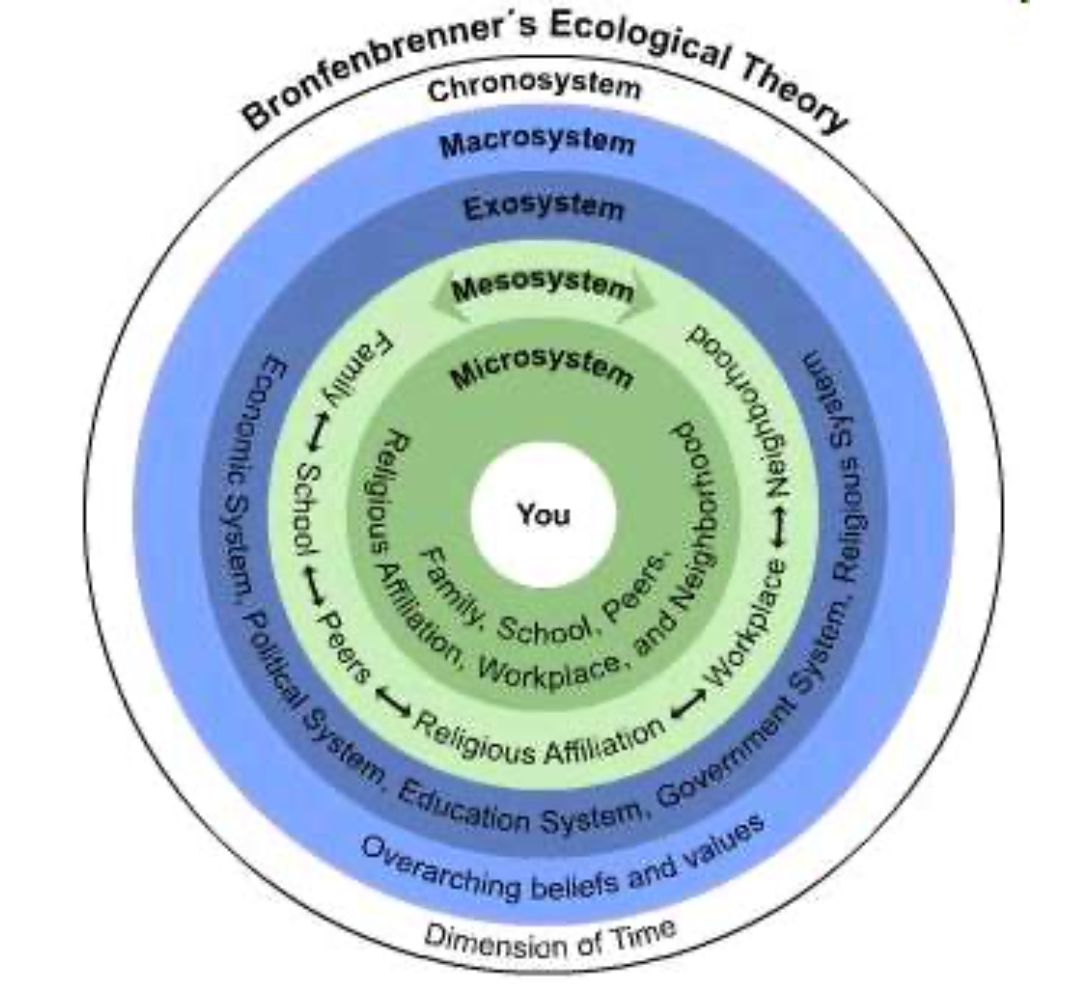
\includegraphics[width=0.6\textwidth]{2-5-eco}
  \caption{Bronferbrenner's Ecological Theory}
  \label{2-5-eco}
\end{figure}
\subsection{Gene-Environment Interaction}
Figure \ref{2-5-iq} shows how our genes might set certain limits on our intelligence, where as the environment determines where we fall in this range. Jerome and Jill are siblings that were separated when they were young and had different upbringings. As such, their IQ range is similar, as they have similar genetics. However, where they ended up within this range is different.
\begin{figure}[htpb]
  \centering
  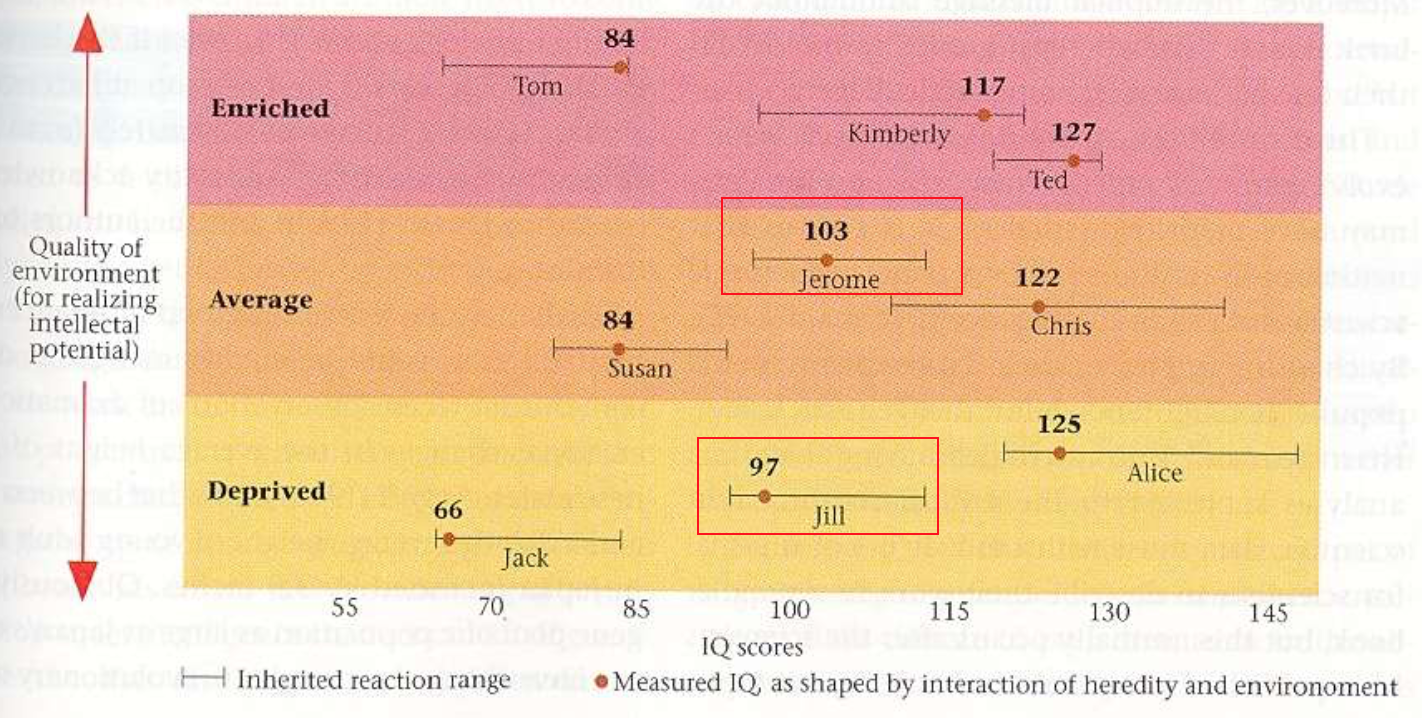
\includegraphics[width=0.6\textwidth]{2-5-iq}
  \caption{Gene-Environment Interaction}
  \label{2-5-iq}
\end{figure}


\begin{definition}
\vocab{Normative influences} are biological or environmental influences that affect many or most people in similar ways
\end{definition}
Normative age-graded changes, e.g. puberty
Normative history-graded changes, major historical events

Non-normative influences.

\end{document}
